\documentclass[14pt,a4paper]{article}
\usepackage[utf8]{inputenc}
\usepackage[russianb]{babel}
\usepackage[left=1.5cm,right=1.5cm,top=2cm,bottom=2.5cm]{geometry}
\usepackage{setspace}
\usepackage{indentfirst}
\usepackage{amssymb}
\usepackage{amsmath}
\usepackage{bm}

\usepackage{array}
\usepackage[pdftex]{graphicx}
\usepackage{comment}
\usepackage[table,xcdraw]{xcolor}


\usepackage{verbatim}


\graphicspath{{images/}}
\renewcommand{\baselinestretch}{1.3}

\begin{document}

Для составления слова КАЗАЧКА нам нужно:
\begin{itemize}
    \item 3 буквы А \\
    \item 2 буквы К \\
    \item 1 буква Ч \\
    \item 1 буква З \\
\end{itemize}

Построим двоичное дерево, чтобы посмотреть, какие коды нам доступны:
\begin{center}
    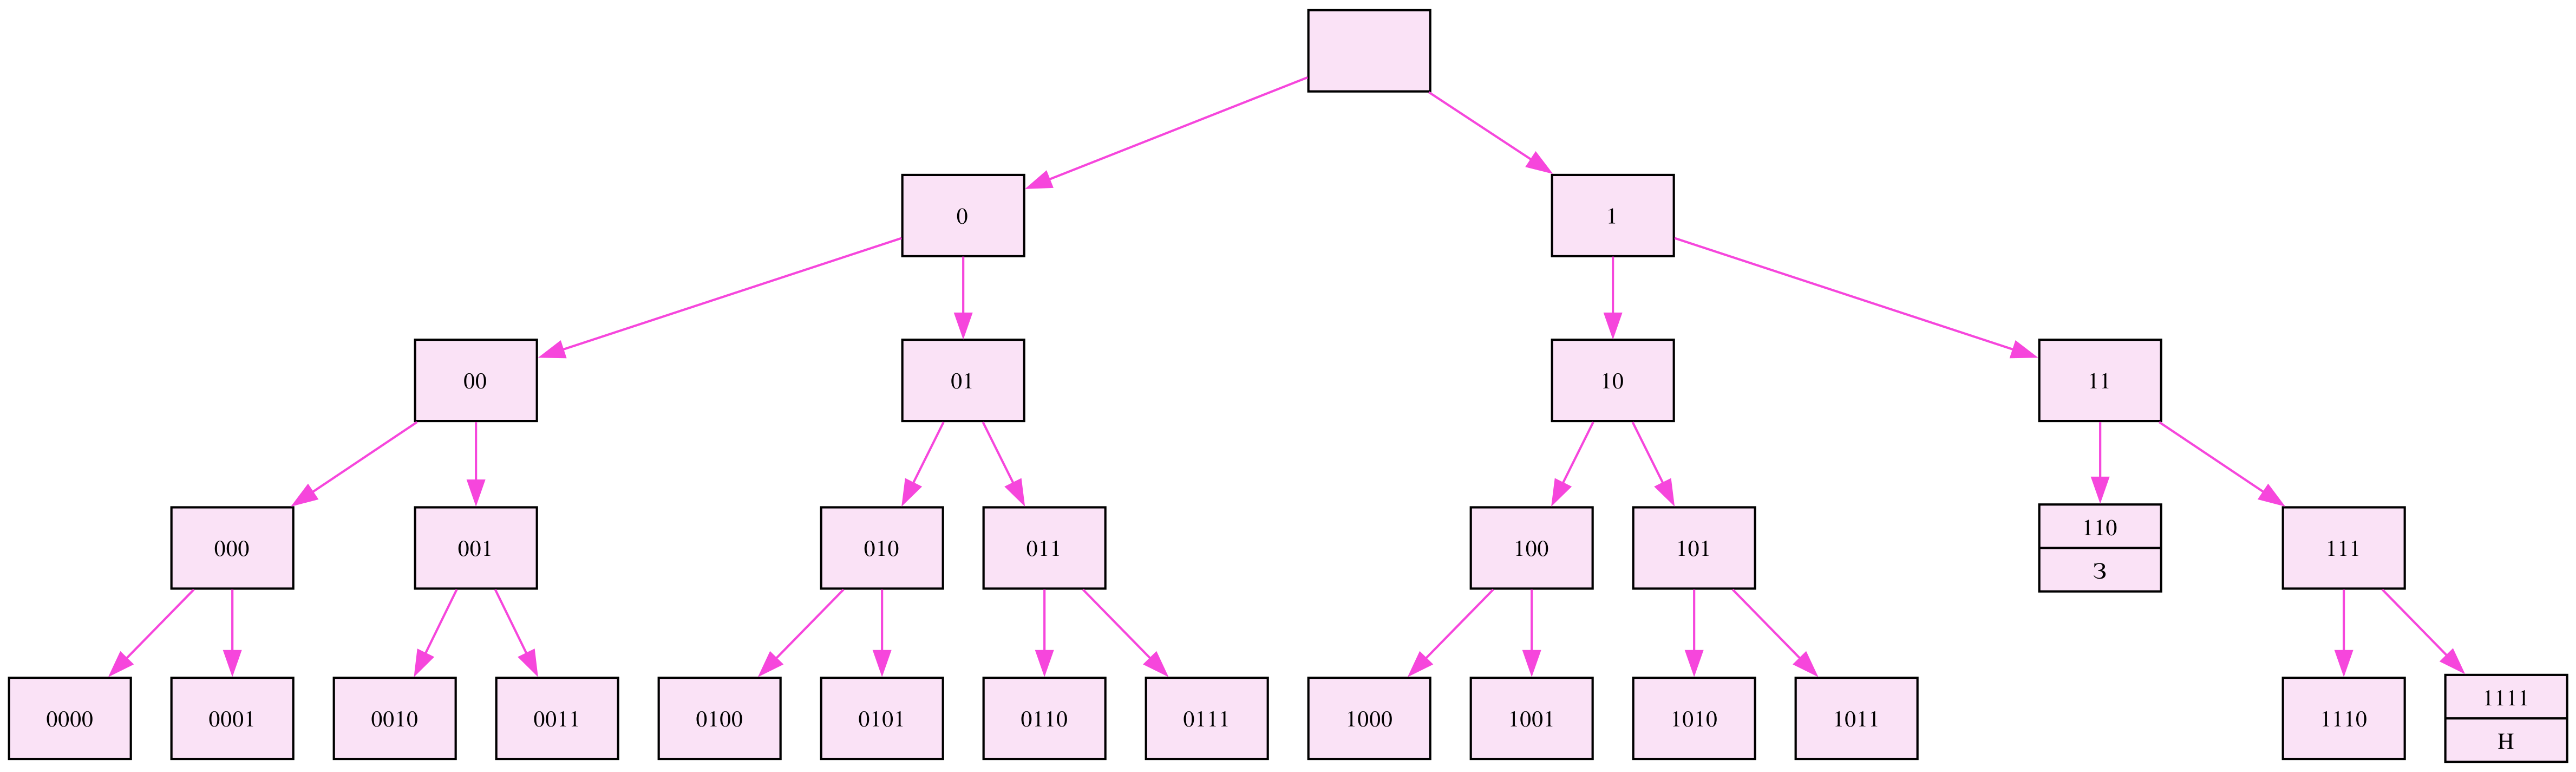
\includegraphics[width=0.5\textwidth]{tree_all.png}
\end{center}

Оптимально взять слеудющие коды:
\begin{itemize}
    \item А -- 0 \\
    \item К -- 10 \\
    \item Ч -- 1110 \\
\end{itemize}
\begin{center}
    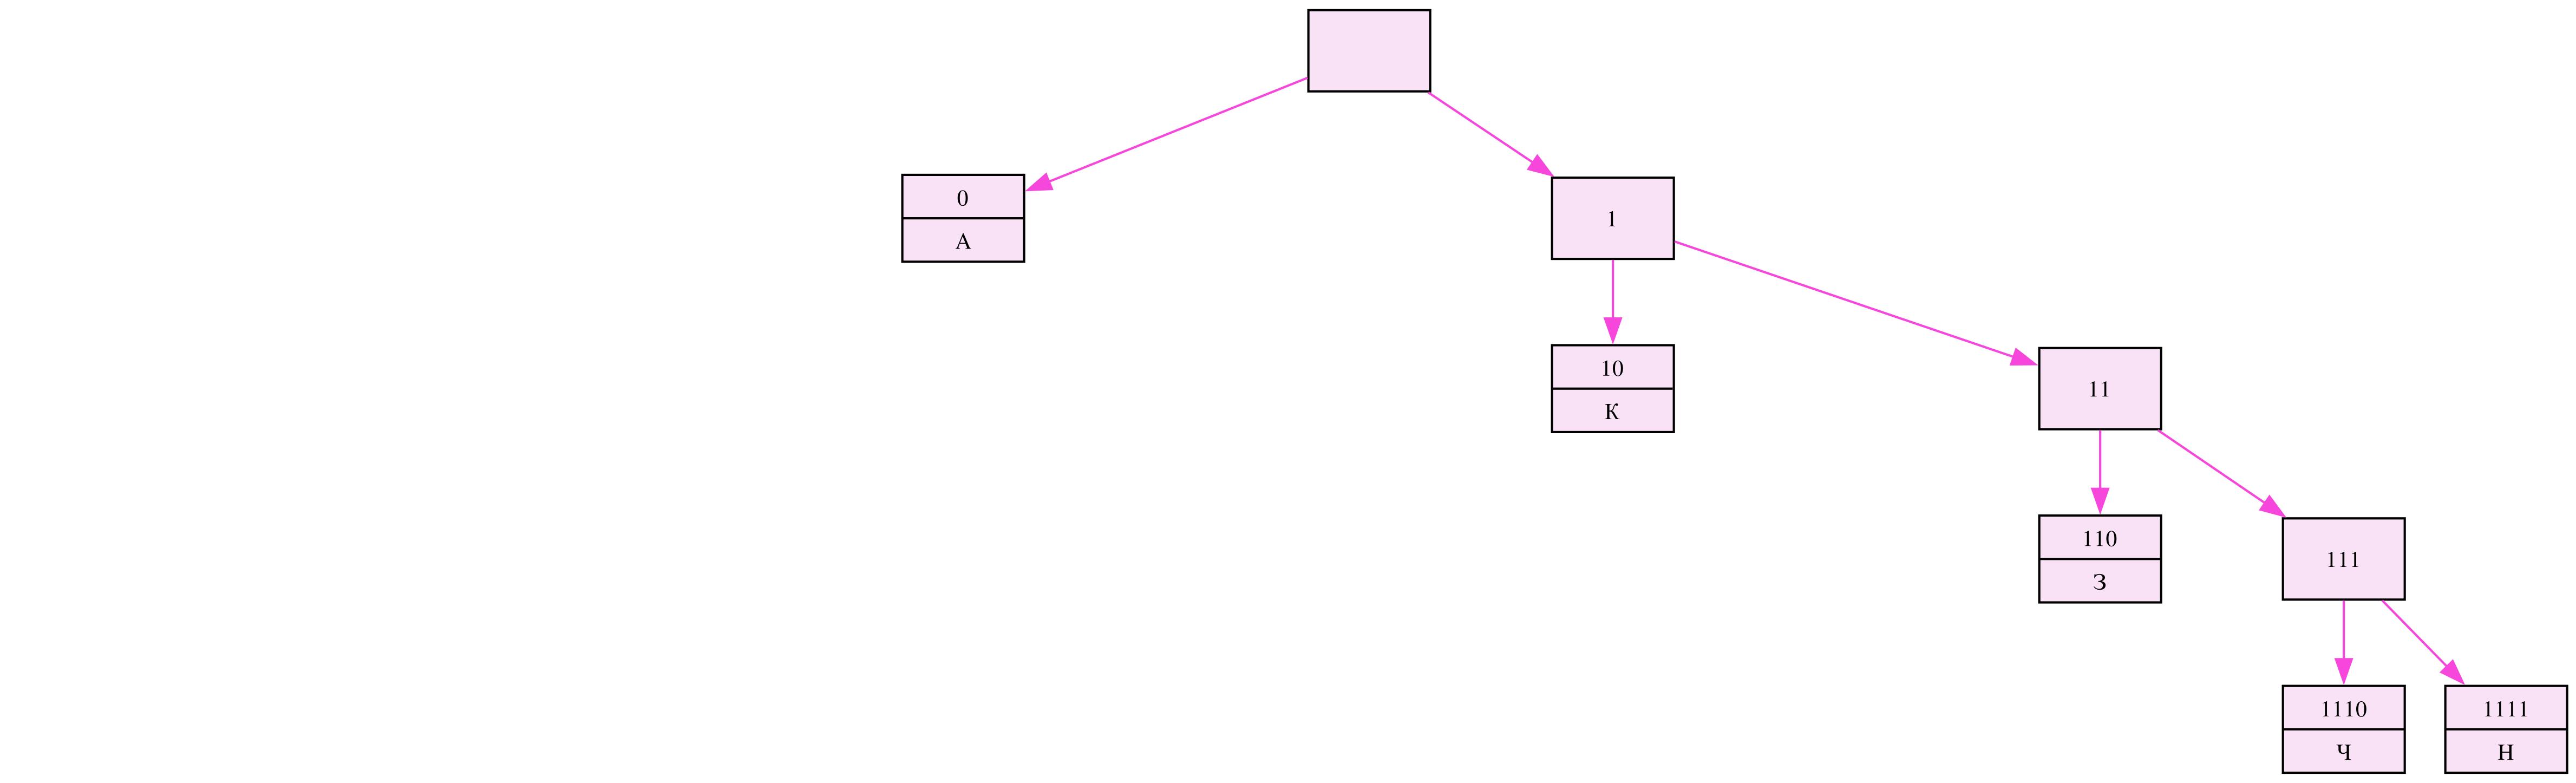
\includegraphics[width=0.5\textwidth]{tree_sol.png}
\end{center}

Тогда КАЗАЧАЧКА закодируется
$3 \cdot 1 + 2 \cdot 2 + 3 + 4 = 14$
знаками.

\end{document}
